%%% Realisering af PWM controller %%%

\subsection{PWM-controller}
I det følgende afsnit testes implementeringen af PWM-controlleren. Her måles frekvensen af savtandspændingen og selve switch-frekvensen, signalet over current-sense modstanden både før og efter filteret, til sidst lave der en gain-fase karakteristik af systemet.

\subsubsection{Switch-frekvens}
Først måles frekvensen af savtandspændingen. Denne frekvens måles til $160k\hertz$, hvor der ønskes $200k\hertz$. Da switch-frekvensen af indflydelse på mange ting i converteren, ændres modstanden således der opnås en frekvens på ca. $200k\hertz$. Der vælges en modstand på $33.2k\ohm$. På figur~\ref{fig:Savtand} og \ref{fig:Udgang_PWM} ses henholdsvis målingen af savtandspændingen og udgangen af PWM-controlleren. Her ses det, at der er opnået en frekvens for savtandspændingen på $192k\hertz$, og en frekvens for udgangssignalet på $102.6k\hertz$. Med et udgangspunkt på $100k\hertz$, godtages denne afvigelse.

\begin{figure}[H]
	\center
	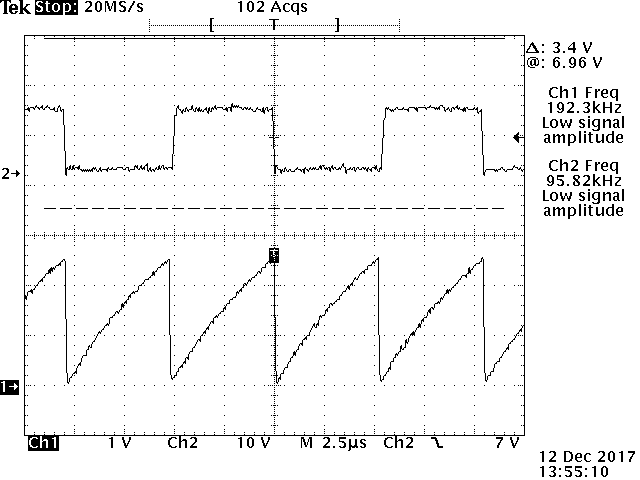
\includegraphics[max width=0.7\linewidth]{/tex/2iteration/billeder/Realisering/Savtand.png}
	\caption{Måling af savtandspænding}
	\label{fig:Savtand}
\end{figure} 

\begin{figure}[H]
	\center
	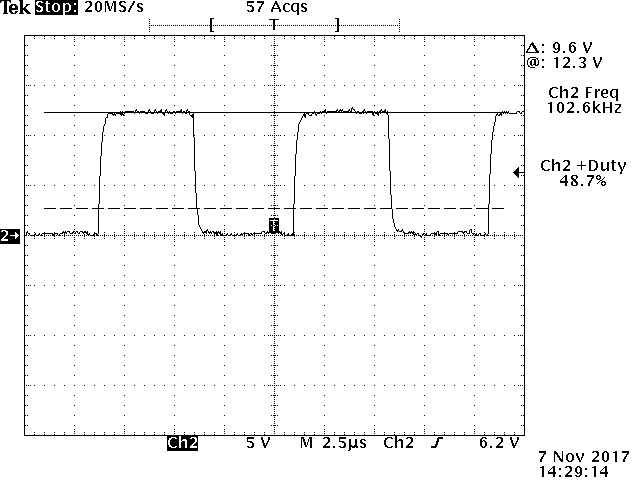
\includegraphics[max width=0.7\linewidth]{/tex/2iteration/billeder/Realisering/Udgang_PWM.png}
	\caption{Udgang af PWM-controller}
	\label{fig:Udgang_PWM}
\end{figure} 

\subsubsection{Current-sense kredsløb}
Current-sense signalet måles både før og efter filteret. Signalet før filteret ses på figur~\ref{fig:CS_U_filter}. Her ses tydeligt de spikes der ønskes filtreret væk, da de overstiger den egentlige peak på signalet. Figur~\ref{fig:CS_M_filter} viser signalet efter filteret. Her ses det at de spikes der var på signalet er blevet filtreret væk. Til gengælder ses det at signalet er blevet langsommere, ved de afrundede hjørner. Dette er ikke optimalt ved lavere duty-cycles, da det som nævnt i afsnit~\ref{CS_protection} vil påvirke systemets I/V-karakteristik. Derfor vil stige tiden af filteret blive optimeret i tredje iteration. 

\begin{figure}[H]
	\center
	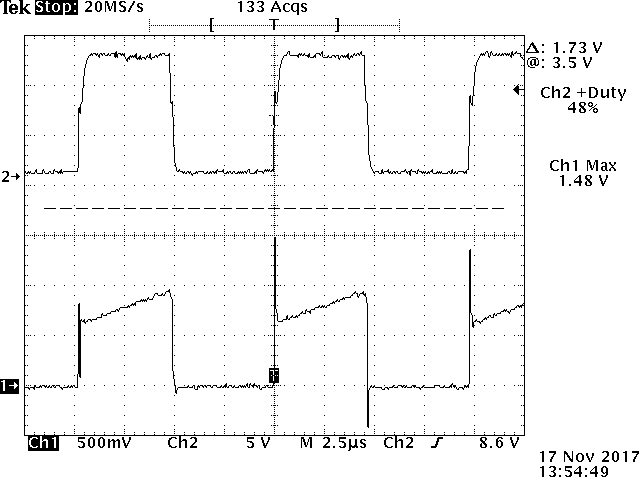
\includegraphics[max width=0.7\linewidth]{/tex/2iteration/billeder/Realisering/CS_U_filter.png}
	\caption{Current-sense signal før filter}
	\label{fig:CS_U_filter}
\end{figure}

\begin{figure}[H]
	\center
	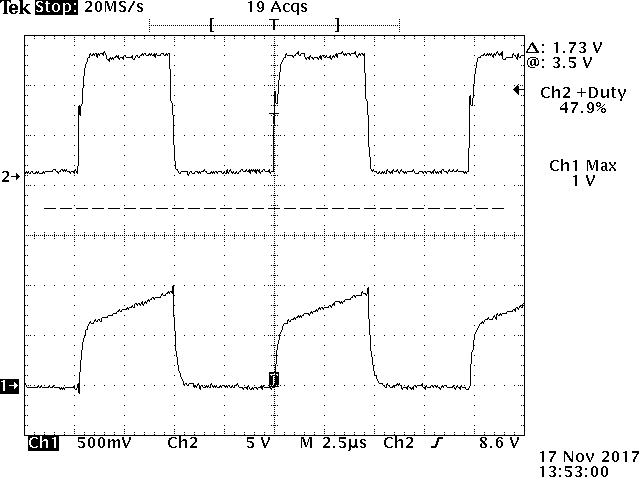
\includegraphics[max width=0.7\linewidth]{/tex/2iteration/billeder/Realisering/CS_M_filter.png}
	\caption{Current-sense signal efter filter}
	\label{fig:CS_M_filter}
\end{figure}


\subsubsection{Spændingsdeler}
Spændingsdeleren testes ved at 

\subsubsection{Gain-fase måling}
Gain-fase målingen deles op i tre, ligesom ved analysen og simuleringen. Der måles overføringsfunktion for power modulet, fejlforstærkeren, og for det samlede system. Målingerne foretages vha. en Network Analyzer af typen HP4194A. Den måler overføringsfunktionen ved at indførere et fejlsignal i tilbagekoblingen, og måle hvordan udgange ændre sig. Derved opnås åbensløjfe overføringsfunktionen. Som ved simuleringen indføres fejlsignalet over en $51.1\ohm$ modstand, placeret i serie med den første modstand i spændingsdeleren. 

Amplituden af fejlsignalet vælges til $30mV$. Ved for lille en amplitude kan signal/støj forholdet blive for småt ved lave frekvenser, mens en stor amplitude kan overstyre fejlforstærkeren. Ud fra Termas erfaringer er $30mV$ et fint udgangspunkt, men den skal muligvis justeres senere. For frekvens-sweepet vælges der et logaritmisk sweep, mens startfrekvensen vælges til $10\hertz$, og slutfrekvensen vælges til $100k\hertz$. 

Først måles gain-fasen for selve power modulet. Det gøres ved at måle mellem udgangen fra fejlforstærkeren, og udgangen fra converteren. Det er vist på figur~\ref{fig:realisering_gain_fase_power}. Der vist bode plot for både analyse og realisering. På grund af usikkerhed i simuleringen er denne del udeladt. Gain for realiseringen er den blå, mens gain for analysen er den grønne stiplede. Fasen for realiseringen er er den røde, mens fasen for analysen er den stiplede lilla. Det ses at gain-fase karakteristikken ser ud som forventet ud fra analysen. Det er først ved de høje frekvenser målingen afviger fra analysen. Båndbredden for power modulet aflæses til ca. $1400\hertz$, mens DC-gain aflæses til ca. $20.3\decibel$.

\begin{figure}[H]
	\center
	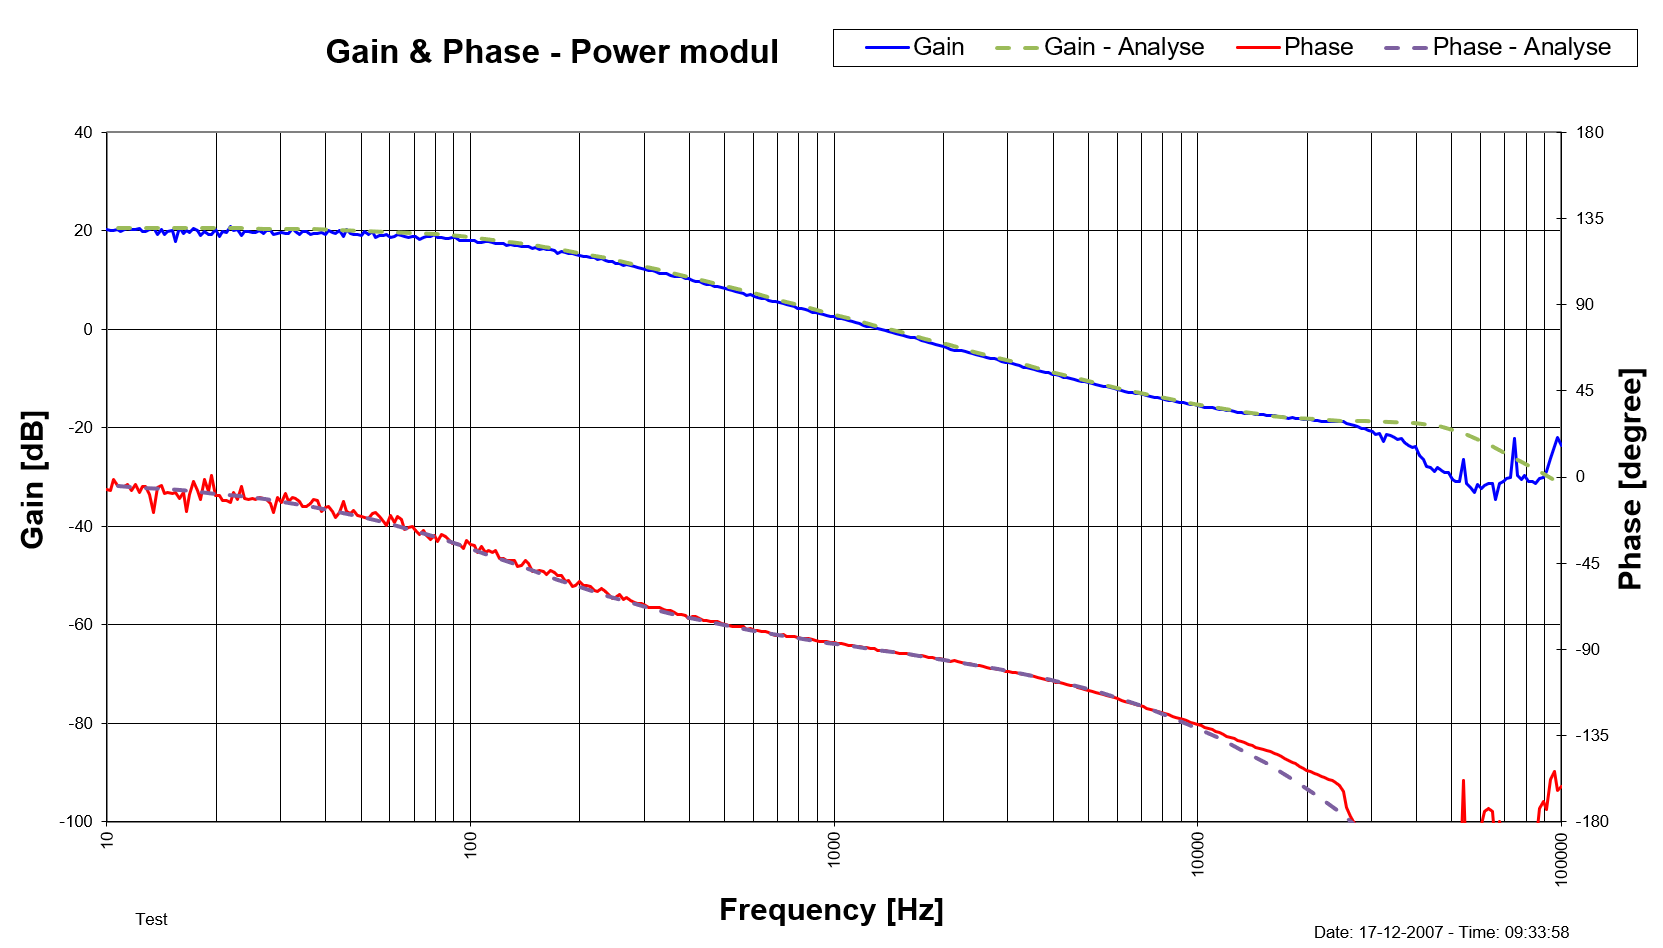
\includegraphics[max width=0.7\linewidth]{/tex/2iteration/billeder/Realisering/Realisering_gain_fase_power.png}
	\caption{Realisering af gain-fase for power modul}
	\label{fig:realisering_gain_fase_power}
\end{figure}

%TODO: Beskriv fejlforstærker når målinger hentes ved Terma


Til sidst måles den samlede overføringsfunktion for systemet. Her måles der over den modstand, hvor fejlsignalet indføres. Det svarer til at måle fra indgangen af fejlforstærkeren til udgangen af converteren. Bode plottet for både analyse og simulering er vist på figur~\ref{fig:realisering_gain_fase_tot}. Gain for realiseringen er den blå, mens gain for analysen er den grønne stiplede. Fasen for realiseringen er er den røde, mens fasen for analysen er den stiplede lilla. På bode plottet ses det at der er en smule større afvigelse, både ved gain og fasen. På trods af afvigelsen aflæses båndbredden dog nogenlunde til det samme på ca. $900\hertz$. Fase-margin aflæses til ca. $62^\circ$, og gain-margin aflæses til ca. $24\decibel$. Holdt op mod analysen var det forventet at opnå en fase-margin på $74.3^\circ$ og en gain-margin på $24\decibel$. Afvigelsen i fase-margin ses på figur~\ref{fig:realisering_gain_fase_tot}, da den faktiske fase ligger under den analyserede. 

\begin{figure}[H]
	\center
	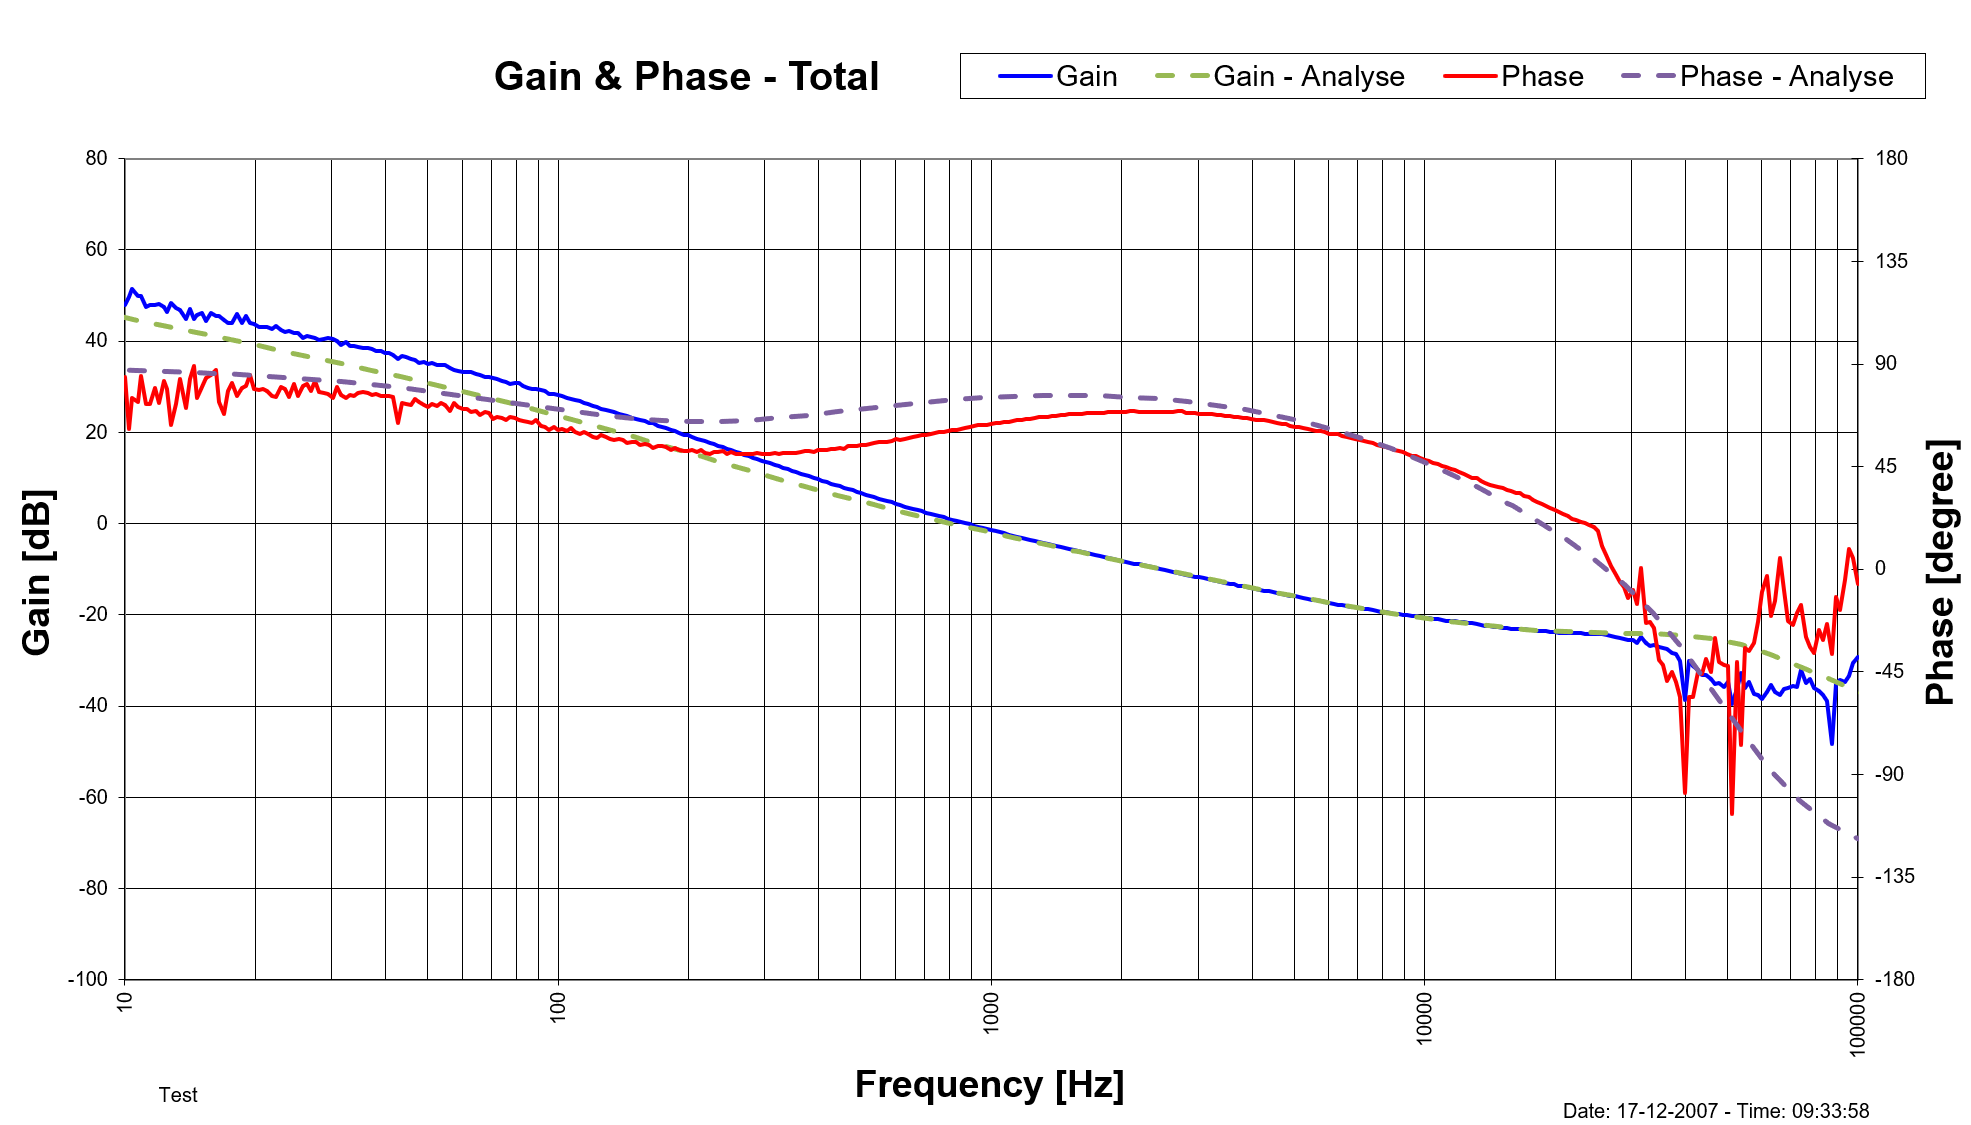
\includegraphics[max width=0.7\linewidth]{/tex/2iteration/billeder/Realisering/Realisering_gain_fase_tot.png}
	\caption{Realisering af gain-fase for hele systemet}
	\label{fig:realisering_gain_fase_tot}
\end{figure}
















